\chapter{Universal Asynchronous Receiver/Transmitter (UART)}\label{ch:sw-uart}

\section{Overview}\label{sec:uart-constr}
\begin{figure}[htbp]
  \centering
  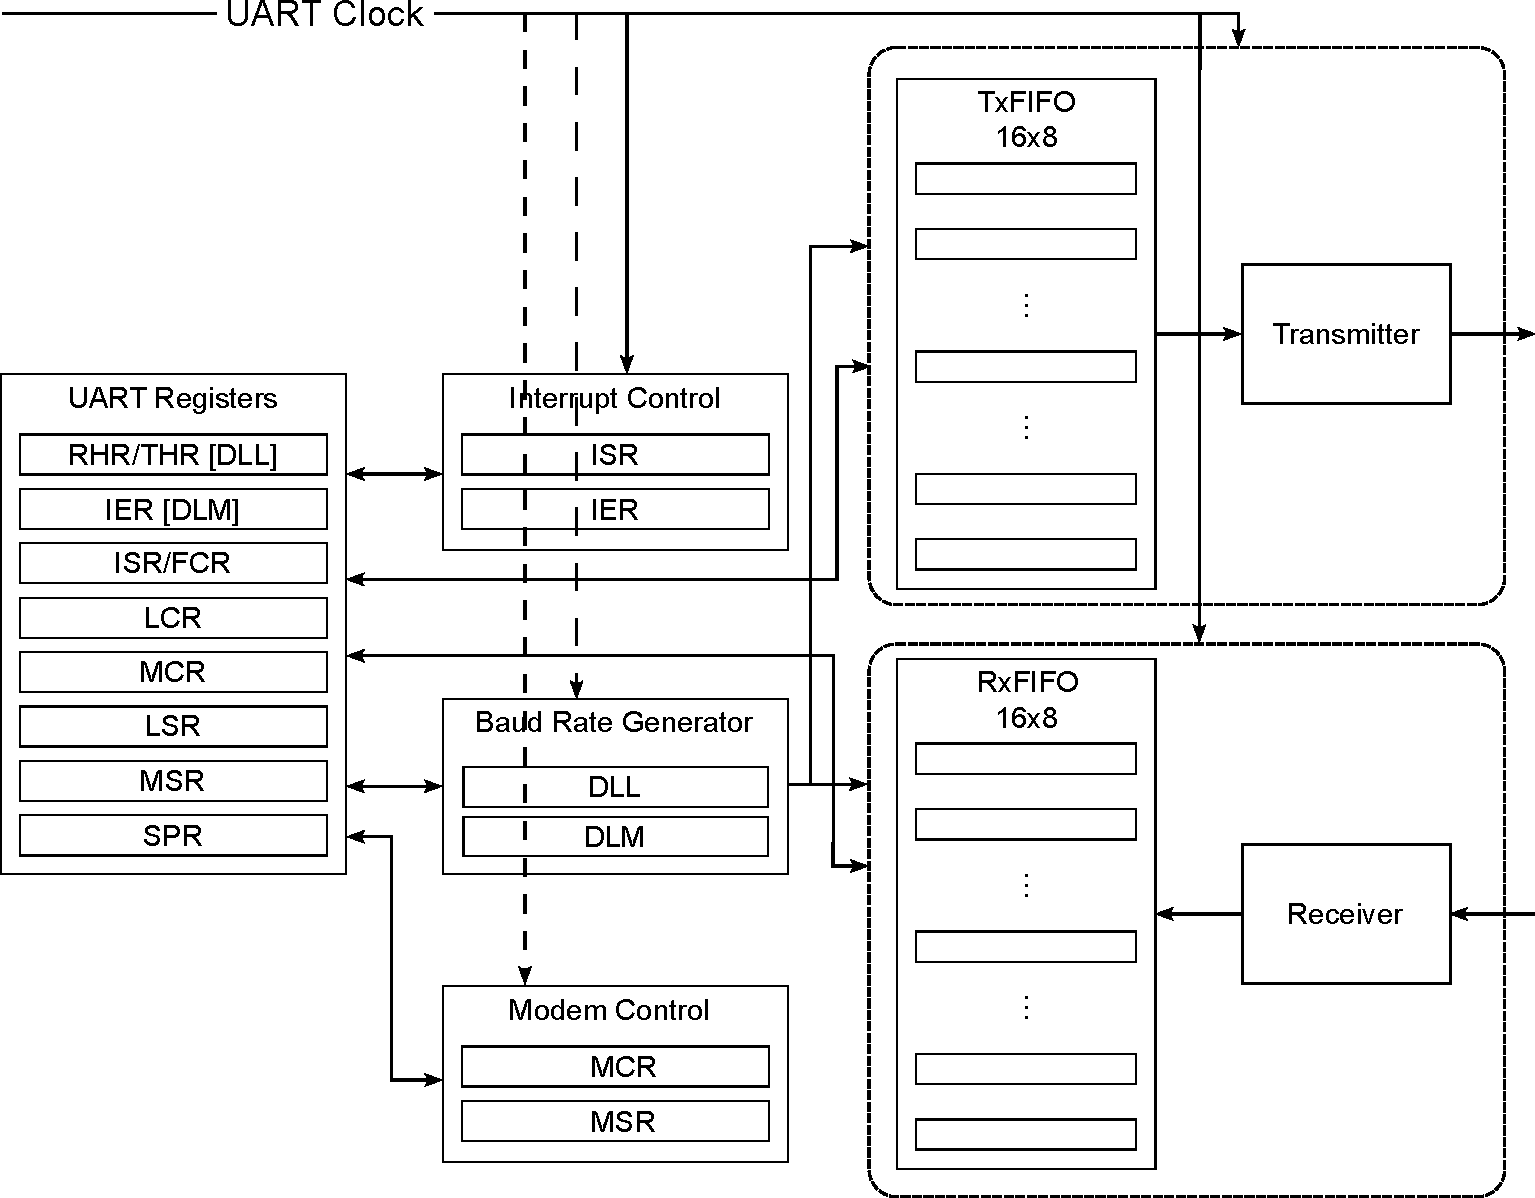
\includegraphics[width=0.85\textwidth]{figures/uart_blk.pdf}
  \caption{UART module high level schematic.}
  \label{fig:obi-uart-schematic}
\end{figure}
The configurator allows the user to add UART modules to either the peripheral cluster in the Pico subsystem or as a part of the NoC subsystem. It is connects to the AHB bus over an AHB to APB bridge that might be shared with any other peripherals in the cluster. \todo{Fix the which UART is used for the NoC sys.}

Both modules provide optional modem control pins as listed in \autoref{tab:uart-modem-signal-list}. 
\begin{table}[htbp]
  \centering
  \begin{tabular}{r l}
    \toprule 
    Signal & Function\footnote{I = Input, O = Output} \\
    \midrule 
    \texttt{cts\_n} & Clear to Send (I)\\
    \texttt{dsr\_n} & Data Send Request (I)\\
    \texttt{ri\_n} & Ring Indicator (I)\\
    \texttt{cd\_n} & Carrier Detect (I)\\
    \texttt{rts\_n} & Ready to Send (O) \\
    \texttt{dtr\_n} & Data Ready (O)\\
    \texttt{out1\_n} & GP signal (optional, O)\\
    \texttt{out2\_n} & GP signal (optional, O)\\
    \bottomrule
  \end{tabular}
  \caption{Optional Modem Control Signals available in the UART module.}
  \label{tab:uart-modem-signal-list}
\end{table}
Use of most signals are implied by their names except, perhaps Ring Indicator and Carrier Detect input signals. These signals (all of them in the table above) are a part of the RS232 Interface specification. The two signals in particular are remnants of the dial-up internet/modem era, and can be safely ignored.  

The modules translate the external AXI/APB interface to a register interface. Registers are byte-addressed on 4-byte boundaries. The 3-bit register index is taken from R/W address bits \texttt{addr[4:2]}:

\[
\texttt{byte\_offset} = \texttt{addr[4:2]} \times 4
\]

The absolute base address is defined by the SoC interconnect (for example, \texttt{0x5000.0000} in Libre-V). Offsets in this document are relative to the UART instance base.

\section{Using the UART}

\subsection{DLAB (Divisor Latch Access Bit)}

Bit~7 of the Line Control Register (\textbf{LCR.DLAB}) multiplexes the mapping at offsets
\texttt{0x00} and \texttt{0x04}:

\begin{itemize}[nosep]
  \item \textbf{DLAB = 0}: normal operation (data and interrupt enable registers).
  \item \textbf{DLAB = 1}: baud-rate divisor latches (\textbf{DLL}, \textbf{DLM}).
\end{itemize}

\subsection{Setting the operating Baud Rate}
To set the baud rate, find the baud rate divisor using:
\[
\mathrm{Divisor} = \frac{\mathrm{SysClkFreq\ (in\ Hz)}}{16 \times \mathrm{Baud\ Rate}}.
\] 
Having found the divisor, you need to quantize it to 16-bits\footnote{The UART currently only supports integer divisors.}. The design generates train of enable pulses based of the provided clock (as opposed to actually dividing the clock signal) based on this divisor. 

To configure the UART, enable the divisor latches by setting \textbf{DLAB = 1}, and set the least significant byte of the 16-bit divisor in \textbf{DLL} and the most significant byte in \textbf{DLM}. 

\subsection{Read/Write Shared Addresses}

Several register names share the same byte offset. The hardware distinguishes them by the
bus transaction direction (\texttt{a.we}):

\begin{itemize}[nosep]
  \item A \textbf{read} at offset \texttt{0x00} returns \textbf{RHR}; a \textbf{write}
        stores \textbf{THR} (when DLAB = 0).
  \item A \textbf{read} at offset \texttt{0x08} returns \textbf{ISR}; a \textbf{write}
        updates \textbf{FCR}.
\end{itemize}

\subsection{FIFOs}

When \textbf{FCR.FIFO\_EN} is set, the transmit and receive paths each use a 16-entry FIFO.
When cleared, only a single-byte holding register is available on each path.

\section{Register Descriptions} 
The following section describes the UART registers in the numerical order of address offset. This section will be useful for those wanting to write custom UART drivers or understand/debug existing drivers. 

\regtitle{0}{Receiver Holding Register (RHR) / Transmitter Holding Register (THR)}

\regmeta{SoC-defined}{0x000}{0x00}{RHR -- RO; THR -- WO}{Read-sensitive (RHR). DLAB must be 0.}

\begin{register}{H}{UART Data Registers RHR/THR}{}

  \regfield[gray!20]{Reserved}{24}{8}{{uninitialized}}
  \regfield{DATA}{8}{0}{00000000}
  \reglabel{Reset}

  \regfieldvalue[gray!20]{Reserved}{24}{8}{{RO}}
  \regfieldvalue{DATA}{8}{0}{{RW}}
  \reglabel{Type}

\end{register}


\textbf{Functional Description.}

Offset \texttt{0x000} is shared by the Receiver Holding Register and the Transmitter Holding Register. A read returns the oldest received data byte from the receive FIFO (if enabled) or from the single-byte RHR. A write pushes a transmit data byte into the transmit FIFO (if enabled) or into the THR; transmission begins automatically when the transmitter is idle.

When DLAB = 1, this offset maps to the Divisor Latch LSB (\textbf{DLL}) instead; see Register~10.

\begin{regmap}
7:0 & DATA & RHR: RO\newline THR: WO & 0 &
Receive/transmit data byte. On read, returns the received character.
On write, loads the next character to transmit. \\
\end{regmap}


\regtitle{1}{Interrupt Enable Register (IER)}

\regmeta{SoC-defined}{0x004}{0x00}{RW}{DLAB must be 0. When DLAB = 1, this offset maps to DLM.}

\begin{register}{H}{UART Intterupt Enable Register (IER)}{}
 
  \regfield[gray!20]{Reserved}{28}{4}{{0}}
  \regfield{MSTAT}{1}{3}{0}
  \regfield{RLTAT}{1}{2}{0}
  \regfield{THRE}{1}{1}{0}
  \regfield{DR}{1}{0}{0}
  \reglabel{Reset}
 
  \regfieldvalue[gray!20]{Reserved}{28}{4}{{RW}}
  \regfieldvalue{MSTAT}{1}{3}{RW}
  \regfieldvalue{RLTAT}{1}{2}{RW}
  \regfieldvalue{THRE}{1}{1}{RW}
  \regfieldvalue{DR}{1}{0}{RW}  
  \reglabel{Type}
 
\end{register}


\textbf{Functional Description.}

The Interrupt Enable Register masks individual interrupt sources. A bit set to 1 allows the
corresponding condition to contribute to the interrupt output \texttt{irq\_o}. Reading or
writing IER does not clear pending interrupts.

\begin{regmap}
7:4 & reserved & RO & 0 &
Reserved. Read as 0. Writes are stored but have no effect. \\
3 & MSTAT & RW & 0 &
Modem Status interrupt enable. When 1, a change in modem status lines may assert an interrupt. \\
2 & RLSTAT & RW & 0 &
Receive Line Status interrupt enable. When 1, overrun, parity, framing, or break errors may
assert an interrupt. \\
1 & THRE & RW & 0 &
Transmitter Holding Register Empty interrupt enable. When 1, an empty THR/TX FIFO may assert
an interrupt. \\
0 & DR & RW & 0 &
Data Ready / Reception Timeout interrupt enable. When 1, received data available or a character
timeout (FIFO mode) may assert an interrupt. \\
\end{regmap}

\regtitle{2}{Interrupt Status Register (ISR)}

\regmeta{SoC-defined}{0x008}{0xC1}{RO}{Read-only. DLAB must be 0.}

\begin{register}{H}{UART Interrupt Status Register (ISR)}{}
 
  \regfield[gray!20]{Reserved}{24}{8}{{0}}
  \regfield{FIFOS\_EN}{2}{6}{11}
  \regfield[gray!20]{Reserved}{2}{4}{{0}}
  \regfield{ID}{3}{1}{000}
  \regfield{STATUS}{1}{0}{1}
  \reglabel{Reset}
 
  \regfieldvalue[gray!20]{Reserved}{24}{8}{{RO}}
  \regfieldvalue{FIFOS\_EN}{2}{6}{{RO}}
  \regfieldvalue[gray!20]{Reserved}{2}{4}{{RO}}
  \regfieldvalue{ID}{3}{1}{{RO}}
  \regfieldvalue{STATUS}{1}{0}{{RO}}
  \reglabel{Type}
 
\end{register}

\textbf{Functional Description.}

The Interrupt Status Register reports whether an interrupt is pending and, if so, the highest
priority interrupt source. The register is implemented in \texttt{obi\_uart\_interrupts.sv}
and is not stored in the main register flip-flop array. Reading ISR identifies the interrupt source but does not by itself clear all interrupt conditions; associated status registers (LSR, MSR, RHR) may need to be serviced.

\begin{regmap}
7:6 & FIFOS\_EN & RO & 2'b11 &
FIFO capability field. Hardwired to \texttt{2'b11} to indicate 16550A-style FIFO support. \\
5:4 & reserved  & RO & 0   & Reserved. Read as 0. \\
3:1 & ID        & RO & 0   &
Interrupt identification code when \textbf{STATUS} = 0:
\begin{itemize}[nosep,leftmargin=*]
  \item \texttt{011}: Receive line status
  \item \texttt{010}: Received data available
  \item \texttt{110}: Character timeout (FIFO mode)
  \item \texttt{001}: THR empty
  \item \texttt{000}: Modem status
\end{itemize} \\
0   & STATUS    & RO & 1   &
Interrupt status. 0 = interrupt pending; 1 = no interrupt pending. \\
\end{regmap}
The ID field is updated in the priority encoder in the interrupt submodule. 

\regtitle{3}{FIFO Control Register (FCR)}

\regmeta{SoC-defined}{0x008}{0x00}{WO}{Write-only. Shares offset with ISR.}

\begin{register}{H}{UART FIFO Control Register (FCR)}{}
 
  \regfield[gray!20]{Reserved}{24}{8}{{0}}
  \regfield{RX\_FIFO\_TL}{2}{6}{00}
  \regfield[gray!20]{Reserved}{3}{3}{{0}}
  \regfield{TX\_FIFO\_RST}{1}{2}{0}
  \regfield{RX\_FIFO\_RST}{1}{1}{0}
  \regfield{FIFO\_EN}{1}{0}{0}
  \reglabel{Reset}
 
  \regfieldvalue[gray!20]{Reserved}{24}{8}{{WO}}
  \regfieldvalue{RX\_FIFO\_TL}{2}{6}{{WO}}
  \regfieldvalue[gray!20]{Reserved}{3}{3}{{WO}}
  \regfieldvalue{TX\_FIFO\_RST}{1}{2}{WO}
  \regfieldvalue{RX\_FIFO\_RST}{1}{1}{WO}
  \regfieldvalue{FIFO\_EN}{1}{0}{WO}
  \reglabel{Type}
 
\end{register}


\textbf{Functional Description.}

The FIFO Control Register configures the on-chip transmit and receive FIFOs that are a part of the UART Tx and Rx submodules. Writes to this
register at offset \texttt{0x008} update FCR; reads at the same offset return ISR.

The RX and TX FIFOs are each 16 entries deep. The RX FIFO stores 11 bits per entry (8 data
bits plus break, framing, and parity error flags). The TX FIFO stores 8-bit characters.

\begin{regmap}
7:6 & RX\_FIFO\_TL      & WO & 0 &
Receive FIFO trigger level:
\begin{itemize}[nosep,leftmargin=*]
  \item \texttt{00}: 1 character
  \item \texttt{01}: 4 characters
  \item \texttt{10}: 8 characters
  \item \texttt{11}: 14 characters
\end{itemize} \\
5:3 & reserved  & WO & 0 & Reserved. \\
2   & TX\_FIFO\_RST & WO & 0 &
Write 1 to reset/clear the transmit FIFO.\\
1   & RX\_FIFO\_RST & WO & 0 &
Write 1 to reset/clear the receive FIFO.\\
0   & FIFO\_EN  & WO & 0 &
FIFO enable. 0 = 8250-style single-byte THR/RHR; 1 = 16550A 16-byte FIFO mode. \\
\end{regmap}


\regtitle{4}{Line Control Register (LCR)}

\regmeta{SoC-defined}{0x00C}{0x00}{RW}{Accessible regardless of DLAB.}

\begin{register}{H}{UART Line Control Register (LCR)}{}
 
  \regfield[gray!20]{Reserved}{24}{8}{{0}}
  \regfield{DLAB}{1}{7}{0}
  \regfield{SBREAK}{1}{6}{0}
  \regfield{SPAR}{1}{5}{0}
  \regfield{EPAR}{1}{4}{0}
  \regfield{PEN}{1}{3}{0}
  \regfield{STP}{1}{2}{0}
  \regfield{WLS}{2}{0}{00}
  \reglabel{Reset}
 
  \regfieldvalue[gray!20]{Reserved}{24}{8}{{RW}}
  \regfieldvalue{DLAB}{1}{7}{{RW}}
  \regfieldvalue{SBREAK}{1}{6}{{RW}}
  \regfieldvalue{SPAR}{1}{5}{{RW}}
  \regfieldvalue{EPAR}{1}{4}{{RW}}
  \regfieldvalue{PEN}{1}{3}{{RW}}
  \regfieldvalue{STP}{1}{2}{{RW}}
  \regfieldvalue{WLS}{2}{0}{{RW}}
  \reglabel{Type}
 
\end{register}


\textbf{Functional Description.}

The Line Control Register defines the serial frame format and the DLAB address-multiplexing
bit. Changes to word length, parity, and stop bits take effect for subsequently transmitted
and received characters.

\begin{regmap}
7   & DLAB      & RW & 0 &
Divisor Latch Access Bit. When 1, offsets \texttt{0x00} and \texttt{0x04} access DLL and DLM.
When 0, they access RHR/THR and IER. \\
6   & SBREAK    & RW & 0 &
Set Break. When 1, forces the transmit output to a spacing (low) condition. \\
5   & SPAR      & RW & 0 &
Stick Parity. When parity is enabled, forces parity bit to 0 (if EPAR = 1) or 1 (if EPAR = 0). \\
4   & EPAR      & RW & 0 &
Even Parity select. 0 = odd parity; 1 = even parity (when parity enabled). \\
3   & PEN       & RW & 0 &
Parity Enable. When 1, a parity bit is transmitted and checked. \\
2   & STP       & RW & 0 &
Stop Bits. 0 = one stop bit; 1 = two stop bits (1.5 stop bits when word length is 5 bits). \\
1:0 & WLS       & RW & 0 &
Word Length Select:
\begin{itemize}[nosep,leftmargin=*]
  \item \texttt{00}: 5 data bits
  \item \texttt{01}: 6 data bits
  \item \texttt{10}: 7 data bits
  \item \texttt{11}: 8 data bits
\end{itemize} \\
\end{regmap}


\regtitle{5}{Modem Control Register (MCR)}

\regmeta{SoC-defined}{0x010}{0x00}{RW}{Accessible regardless of DLAB.}

\begin{register}{H}{UART Modem Control Register (MCR)}{}
 
  \regfield[gray!20]{Reserved}{24}{8}{{0}}
  \regfield[gray!20]{Reserved}{3}{5}{{0}}
  \regfield{LOOP}{1}{4}{0}
  \regfield{OUT2}{1}{3}{0}
  \regfield{OUT1}{1}{2}{0}
  \regfield{RTS}{1}{1}{0}
  \regfield{DTR}{1}{0}{0}
  \reglabel{Reset}
 
  \regfieldvalue[gray!20]{Reserved}{24}{8}{{RW}}
  \regfieldvalue[gray!20]{Reserved}{3}{5}{{RO}}
  \regfieldvalue{LOOP}{1}{4}{RW}
  \regfieldvalue{OUT2}{1}{3}{RW}
  \regfieldvalue{OUT1}{1}{2}{RW}
  \regfieldvalue{RTS}{1}{1}{RW}
  \regfieldvalue{DTR}{1}{0}{RW}
  \reglabel{Type}
 
\end{register}

\textbf{Functional Description.}

The Modem Control Register drives modem output pins and enables internal loopback for test.
Modem outputs are active-low on the external pins (\texttt{rts\_no}, \texttt{dtr\_no}, etc.).

\begin{regmap}
7:5 & reserved  & RO & 0 & Reserved. Read as 0. \\
4   & LOOP      & RW & 0 &
Loopback. When 1, the transmitter output is looped back to the receiver input internally. \\
3   & OUT2      & RW & 0 & Auxiliary output 2 (optional GPIO). \\
2   & OUT1      & RW & 0 & Auxiliary output 1 (optional GPIO). \\
1   & RTS       & RW & 0 & Request To Send output. \\
0   & DTR       & RW & 0 & Data Terminal Ready output. \\
\end{regmap}

\regtitle{6}{Line Status Register (LSR)}

\regmeta{SoC-defined}{0x014}{0x60}{RO}{Read-sensitive. DLAB must be 0.}

\begin{register}{H}{UART Line Status Register (LSR)}{}
 
  \regfield[gray!20]{Reserved}{24}{8}{{0}}
  \regfield{FIFO\_ERR}{1}{7}{0}
  \regfield{TXE}{1}{6}{1}
  \regfield{THRE}{1}{5}{1}
  \regfield{BI}{1}{4}{0}
  \regfield{FE}{1}{3}{0}
  \regfield{PE}{1}{2}{0}
  \regfield{OE}{1}{1}{0}
  \regfield{DR}{1}{0}{0}
  \reglabel{Reset}
 
  \regfieldvalue[gray!20]{Reserved}{24}{8}{{RO}}
  \regfieldvalue{FIFO\_ERR}{1}{7}{RO}
  \regfieldvalue{TXE}{1}{6}{RO}
  \regfieldvalue{THRE}{1}{5}{RO}
  \regfieldvalue{BI}{1}{4}{RO}
  \regfieldvalue{FE}{1}{3}{RO}
  \regfieldvalue{PE}{1}{2}{RO}
  \regfieldvalue{OE}{1}{1}{RO}
  \regfieldvalue{DR}{1}{0}{RO}
  \reglabel{Type}
 
\end{register}


\textbf{Functional Description.}

The Line Status Register provides transmit readiness and receive status, including error
flags. Unlike some UART designs, error information is \emph{not} embedded in the RHR read
data; errors are reported only in LSR. Reading LSR clears the receive-line-status interrupt. Individual error bits are cleared on
LSR read when no additional FIFO errors remain.

\begin{regmap}
7   & FIFO\_ERR   & RO & 0 &
FIFO Error. Set when at least one character with an error was received into the RX FIFO. \\
6   & TXE    & RO & 1 &
Transmitter Empty. 1 when the transmitter shift register and holding logic are completely idle. \\
5   & THRE    & RO & 1 &
THR Empty. 1 when the THR or TX FIFO can accept a new write. \\
4   & BI      & RO & 0 &
Break Indicator. 1 when a break condition was detected on the receive line. \\
3   & FE      & RO & 0 &
Framing Error. 1 when the stop bit was not received as expected. \\
2   & PE      & RO & 0 &
Parity Error. 1 when the received parity bit did not match. \\
1   & OE      & RO & 0 &
Overrun Error. 1 when a new character arrived before the previous one was read (RHR mode) or
when the RX FIFO was full (FIFO mode). \\
0   & DR      & RO & 0 &
Data Ready. 1 when received data is available in RHR or the RX FIFO. \\
\end{regmap}


\regtitle{7}{Modem Status Register (MSR)}

\regmeta{SoC-defined}{0x018}{0x00}{RO}{Read-sensitive. DLAB must be 0.}

\begin{register}{H}{UART Modem Status Register (MSR)}{}
 
  \regfield[gray!20]{Reserved}{24}{8}{{0}}
  \regfield{CD}{1}{7}{0}
  \regfield{RI}{1}{6}{0}
  \regfield{DSR}{1}{5}{0}
  \regfield{CTS}{1}{4}{0}
  \regfield{DCD}{1}{3}{0}
  \regfield{TERI}{1}{2}{0}
  \regfield{DDSR}{1}{1}{0}
  \regfield{DCTS}{1}{0}{0}
  \reglabel{Reset}
 
  \regfieldvalue[gray!20]{Reserved}{24}{8}{{RO}}
  \regfieldvalue{CD}{1}{7}{RO}
  \regfieldvalue{RI}{1}{6}{RO}
  \regfieldvalue{DSR}{1}{5}{RO}
  \regfieldvalue{CTS}{1}{4}{RO}
  \regfieldvalue{DCD}{1}{3}{RO}
  \regfieldvalue{TERI}{1}{2}{RO}
  \regfieldvalue{DDSR}{1}{1}{RO}
  \regfieldvalue{DCTS}{1}{0}{RO}
  \reglabel{Type}
 
\end{register}


\textbf{Functional Description.}

The Modem Status Register reports the state of modem input signals and edge-detected changes.
Delta bits (bits 4--7 in this implementation) are sticky and remain set until MSR is read.

Modem input pins are active-low externally; the register stores the logical (non-inverted)
levels and change indicators.

\begin{regmap}
7   & CD    & RO & 0 & Carrier Detect input level. \\
6   & RI    & RO & 0 & Ring Indicator input level. \\
5   & DSR   & RO & 0 & Data Set Ready input level. \\
4   & CTS   & RO & 0 & Clear To Send input level. \\
3   & DCD  & RO & 0 & Delta Carrier Detect. Set when CD input changes state. \\
2   & TERI  & RO & 0 & Trailing Edge Ring Indicator. Set on high-to-low transition of RI. \\
1   & DDSR  & RO & 0 & Delta Data Set Ready. Set when DSR input changes state. \\
0   & DCTS  & RO & 0 & Delta Clear To Send. Set when CTS input changes state. \\
\end{regmap}


\regtitle{8}{Scratch Pad Register (SPR)}

\regmeta{SoC-defined}{0x01C}{0x00}{RO}{Not implemented.}

\begin{register}{H}{UART Scratch Pad Register (SPR)}{}
 
  \regfield[gray!20]{Reserved}{24}{8}{{0}}
  \regfield{DATA}{8}{0}{00000000}
  \reglabel{Reset}
 
  \regfieldvalue[gray!20]{Reserved}{24}{8}{{RO}}
  \regfieldvalue{DATA}{8}{0}{{RO}}
  \reglabel{Type}
 
\end{register}


\textbf{Functional Description.}

The optional Scratch Pad Register is defined by the 16550A standard as a software-writable storage
location. In this implementation, reads always return \texttt{0x00} and writes are silently
ignored. No error is generated.

\begin{regmap}
7:0 & DATA & RO & 0 & Always reads zero. Writes have no effect. \\
\end{regmap}


\regtitle{9}{Divisor Latch LSB (DLL)}

\regmeta{SoC-defined}{0x000}{0x01}{RW}{DLAB must be 1. Shares offset with RHR/THR.}

\begin{register}{H}{UART Divisor Latch LSB (DLL)}{}
 
  \regfield[gray!20]{Reserved}{24}{8}{{uninitialized}}
  \regfield{DIV\_LSB}{8}{0}{00000001}
  \reglabel{Reset}
 
  \regfieldvalue[gray!20]{Reserved}{24}{8}{{RO}}
  \regfieldvalue{DIV\_LSB}{8}{0}{{RW}}
  \reglabel{Type}
 
\end{register}


\textbf{Functional Description.}

When DLAB = 1, offset \texttt{0x000} maps to the least significant byte of the 16-bit baud
rate divisor. The divisor is combined with DLM as:

% \[
% \mathrm{divisor} = \{\mathrm{DLM}, \mathrm{DLL}\}, \qquad
% \mathrm{baud} = \frac{f_{\mathrm{clk}}}{16 \times \mathrm{divisor}}
% \]

A divisor of 0 is invalid and disables baud-rate generation. Writing DLL or DLM resets the
internal baud counters.

\begin{regmap}
7:0 & DIV\_LSB & RW & 0x01 & Least significant byte of the baud divisor latch. \\
\end{regmap}


\regtitle{10}{Divisor Latch MSB (DLM)}

\regmeta{SoC-defined}{0x004}{0x00}{RW}{DLAB must be 1. Shares offset with IER.}

\begin{register}{H}{UART Divisor Latch MSB (DLM)}{}
  \regfield[gray!20]{Reserved}{24}{8}{{0}}
  \regfield{DIV\_MSB}{8}{0}{00000000}
  \reglabel{Reset}
  \regfieldvalue[gray!20]{Reserved}{24}{8}{{RW}}
  \regfieldvalue{DIV\_MSB}{8}{0}{{RW}}
  \reglabel{Type}

\end{register}


\textbf{Functional Description.}

When DLAB = 1, offset \texttt{0x004} maps to the most significant byte of the baud rate
divisor. See Register~9 for the baud-rate formula.

\begin{regmap}
7:0 & DIV\_MSB & RW & 0x00 & Most significant byte of the baud divisor latch. \\
\end{regmap}


\subsection{Address Map Summary}

\begin{tabular}{@{}lllll@{}}
\toprule
\textbf{Offset} & \textbf{DLAB = 0 (read)} & \textbf{DLAB = 0 (write)} &
\textbf{DLAB = 1 (read)} & \textbf{DLAB = 1 (write)} \\
\midrule
0x000 & RHR & THR & DLL & DLL \\
0x004 & IER & IER & DLM & DLM \\
0x008 & ISR & FCR & ISR & FCR \\
0x00C & LCR & LCR & LCR & LCR \\
0x010 & MCR & MCR & MCR & MCR \\
0x014 & LSR & --- & --- & --- \\
0x018 & MSR & --- & --- & --- \\
0x01C & SPR & SPR & SPR & SPR \\
\bottomrule
\end{tabular}

\newpage
